\begin{frame}
  \frametitle{Method of Characteristics}
    \begin{columns}
      \column[t]{5cm}
        The method of characteristics (MOC) is a numerical technique for solving PDE's,
        including the NTE. 
        
        MOC transforms our spatially 3D PDE into a spatially 1D PDE by
        transforming the problem's spatial domain from $\mathbb{R}^{3}$
        to $\mathcal{R}_k$, where
        \begin{equation}
            \label{eq:R_k}
            \mathcal{R}_k = \{\vec{r}_k \in \mathbb{R}^3 : \vec{r_k} = \vec{r}_n + s \hat{\Omega}_k \}
        \end{equation}
        for a specific reference position $\vec{r}_n$ and ordinate $\hat{\Omega}_k$.
        
        This {\it characteristic transform} changes the streaming operator as
        $\hat{\Omega} \cdot \nabla
        \rightarrow \pps$, where $s_k$ is the $s$ parameter corresponding to
        characteristic $\vec{r}_k$

      \column[t]{5cm}
        \begin{figure}[htbp!]
          \begin{center}
            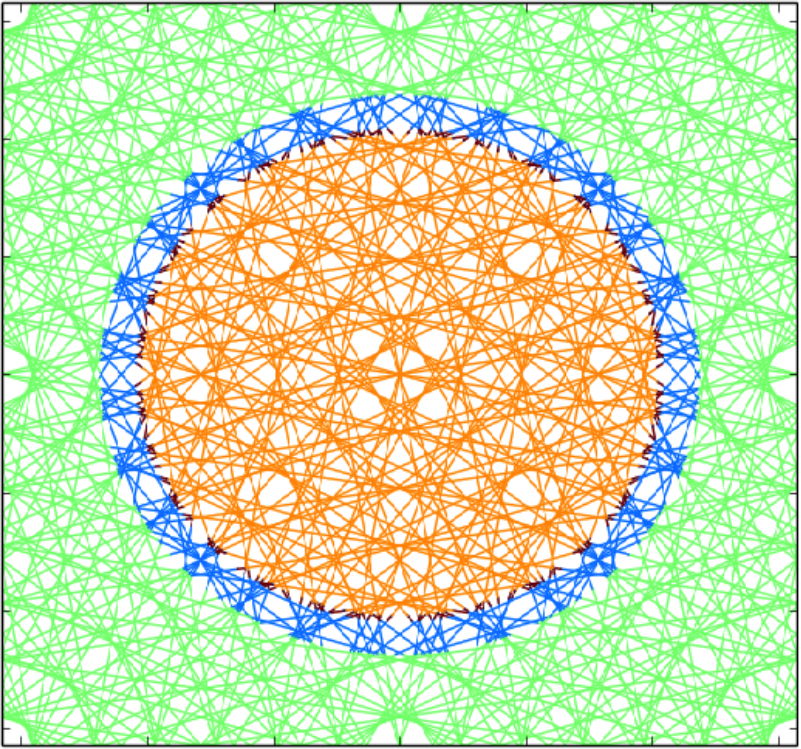
\includegraphics[height=4cm]{./figs/tramm-csg-tracks.png}
          \end{center}
          \caption{Precomputed set of tracks used in MOC, called a {\it track
          laydown}. Reproduced from \cite{tramm_development_2018}.}
          \label{fig:moc-tracks}
        \end{figure}
      \end{columns}
\end{frame}
